% !TeX encoding = UTF-8
% !TeX program = pdflatex
% !BIB program = biber

%%% To write an article in English, please use the option ``english'' in order
%%% to get the correct hyphenation patterns and terms.
%%% \documentclass[english]{class}
%%% for anonymizing an article you can use the ``anonymous'' option.
%%%
%%% Um einen Artikel auf deutsch zu schreiben, genügt es die Klasse ohne
%%% Parameter zu laden.
%%% Zur Anonymisierung kann die ``anonymous'' Option genutzt werden.
\documentclass[english]{lni}
\usepackage{dirtytalk}
\usepackage{graphicx}

%%
\begin{document}
%%% Mehrere Autoren werden durch \and voneinander getrennt.
%%% Die Fußnote enthält die Adresse sowie eine E-Mail-Adresse.
%%% Das optionale Argument (sofern angegeben) wird für die Kopfzeile verwendet.
\title[Ein Kurztitel]{Exposé for the Master's Thesis \textit{Augmenting Enterprise Architecture Landscapes with AI: A Retrieval-Augmented Chatbot Approach using Graph Databases}}
%% \subtitle{Untertitel / Subtitle} % if needed
 \author[1]{Hendrik Gruber}{hendrik.gruebr@stud.fra-uas.de}{}
 \affil[1]{Frankfurt Univeristy of Applied Sciences}
\maketitle

%\begin{abstract}
%Dies ist eine kurze Übersicht über das Dokument mit einer Länge von
%70 bis 150 Wörtern. Es sollte ein Absatz sein, der die relevantesten
%Aspekte enthält.
%\end{abstract}


This exposé outlines what, why, and how the work for my planned master's thesis will be conducted. The goal of this exposé is to provide an overview of the subject matter and to demonstrate my understanding of the research topic.

\begin{keywords}
AI chatbot, Retrieval-Augmented Generation (RAG), Enterprise Architecture Management (EAM).
\end{keywords}
%%% Beginn des Artikeltexts
%\section{Überschrift/Heading}


\section{Problem Statement and Research Questions}
Within the realm of Enterprise Architecture Management (EAM), updating and maintaining the architecture landscape when new projects or applications arise can be a tedious task. It requires that the Enterprise Architect (EA) understands the landscape of existing projects and applications and the changes required to reflect these new, incoming initiatives in a way that preserves consistency, avoids redundancies in the landscape, and supports the organization's strategic goals. Because the landscape of a company can be highly complex, containing hundreds of applications and projects, seeing the big picture can be a difficult task for an individual or even for an entire team. \textbf{todo Quelle}

This is a laborious task which can potentially be supplemented with the help of generative AI \textbf{todo Quelle}. AI can read in application and project descriptions written in natural language and map this information against the existing data. However, as it stands, there is a lack of GenAI solutions for this specific problem. All existing solutions either have outdated models or are only theoretical work.

The master's thesis will be tackling the following research question: \say{\textbf{How can generative AI support Enterprise Architects in assessing the impact of new or changing projects on the application landscape?}} Three supplementary questions will be answered when approaching the main thesis questions:
\begin{enumerate}
    \item \say{What are the current challenges faced by Enterprise Architects when updating landscapes with new projects?}
    \item \say{What are the current challenges faced by Enterprise Architects when updating landscapes with new projects?}
    \item \say{How can project descriptions be transformed into graph-based representations that integrate with existing landscapes?}
    \item \say{How effective is a generative AI chatbot in supporting Enterprise Architects compared to traditional EAM tools?}
\end{enumerate}


\section{Methodology and Approach}
Test lorem ipsum si dolor et amet \cite{ettinger2025enterprise}

\begin{figure}[h]
\centering
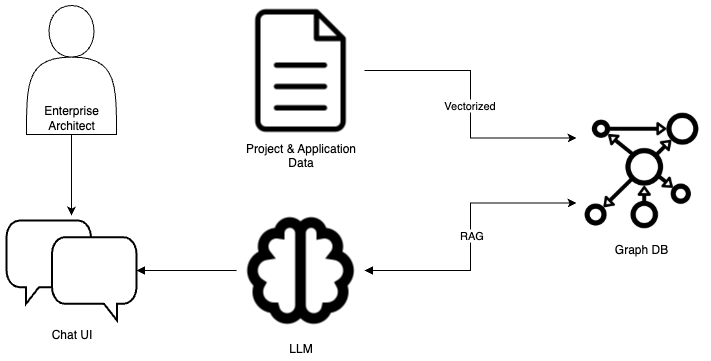
\includegraphics[scale=0.5]{./architecture_diagram.png}
\caption{A first draft architecture diagram of the expected system components and points of interaction between them.}
\end{figure}

\section{Expected Contribution}
Test lorem ipsum si dolor et amet \cite{ettinger2025enterprise}

\section{Thesis Outline and Structure}
\begin{itemize}
    \item Introduction, Motivation, and Thesis Question
    \item Background Information and Literature
    \item Current State of the Art
    \item Methodology
    \item Evaluation of the Results, Discussion, and Challenges Faced
    \item Conclusion and Future Work
\end{itemize}




\printbibliography
\end{document}
